\subsection{Air Traffic Control}\label{sec:AirTrafficControl}
\paragraph{Motivation:} The modern \emph{Air Traffic Control} (ATC) procedures are outlined in ICAO 4444 \cite{icao4444}. The ATC roles and responsibilities regarding \emph{clearance}, \emph{self-separation}, and, \emph{provided traffic information} are summarized in (tab. \ref{tab:airspaceResponsibilitiesIcao}). 

The \emph{main role} of \emph{Air Traffic Control} (ATC) is to support the organization of the \emph{airspace} concerning \emph{preemptive} detect and avoid.

\begin{note}
    The \emph{Reactive} and \emph{Event-Based} detect and avoid for manned aviation are covered by \emph{ACAS-X/TCAS systems} (sec. \ref{sec:ACASX}, \ref{sec:TCAS})
\end{note}

\paragraph{Commands issued by ATC:} There are multiple levels of commands issued by ATC, their characteristics and the compulsory level is defined as folows:

\begin{enumerate}
    \item \emph{Notification} - the information notification, commonly known as \emph{NoTice to AirMan} (NOTAM), depending on flight mode, can be transmitted as a voice message or information broadcast. They usually contain information about weather and traffic situation in the given sector.
    
    \item \emph{Warning} - directed message to specific general aviation  which may require some direct action. The information is usually informative, but the action is not mandatory.
    
    \item \emph{Recommendation} - directed a message to specific general aviation  which requires direct action. The order is usually a specific action, but the action is not mandatory to be executed by the pilot.
    
    \item \emph{Directive} - directed a message to specific general aviation  which requires direct action. The order is specific action, and the order fulfillment is mandatory for the pilot. 
\end{enumerate}

\paragraph{Separation enforcement:} The \emph{separation} is the main feature of the ATC in controlled airspace of airports (B, C, D class). Its enforced by the management of \emph{action clearance}. The ATC issues the clearance for take-off/landing sequence. 

The clearance for climb/descent is given at the beginning when the flight plan is approved. The ATC issues the time slots for selected pathways. The continuous monitoring of air traffic is executed in periods. The airplane deviation from the cleared plan should be minimal. 

If there is any incident the \emph{ATC} can take the following actions:
\begin{enumerate}
    
    \item \emph{Heading change} - order \emph{general aviation} to change heading in a given time frame (horizontal navigation). This command is usually issued to correct horizontal deviations in path tracking.
    
    \item \emph{Velocity change} - order \emph{general aviation} to change velocity in a given time frame. This command is usually issued to correct time deviations in path tracking.
    
    \item \emph{Altitude change} (Flight Level) - order \emph{general aviation} to climb or descent in a given time frame. This command is usually issued to correct vertical deviations in path tracking (wrong flight level).
    
    \item \emph{Divergence} - order \emph{general aviation} to follow different waypoint in flight plan (goal change). This command is usually used to resolve incidents or to reroute traffic to another hub.
    
    \item \emph{Convergence} - order \emph{general aviation} to return to following original waypoint (goal return). This command is usually used when incident has been resolved in a short time, and the original flight \emph{path} can be re-established.
    
    \item \emph{Restrictions Enforcement} - order \emph{general aviation} to avoid some point with defined distance.  
\end{enumerate}

\begin{note}
    All ATC commands can be requested be \emph{general aviation} for clearance to be granted. Meaning the airplane can ask ATC to perform any of the listed actions. 
\end{note}

The \emph{separation} can be divided into two distinct types to form \emph{well clear barrel} (fig. \ref{fig:WellClearTreshold}). The separation types are the following:

\begin{enumerate}
    \item \emph{Horizontal separation} - keep clear of any intruders on the horizontal plane (flight level plane).
    
    \item \emph{Vertical separation} - keep clear of any intruders on given altitude (flight level) range.
\end{enumerate}

\begin{note}
    The \emph{horizontal/vertical} separation is enforced independently, reducing 3D avoidance problem to 2D/1D avoidance problem.
\end{note}

\paragraph{Traffic Information:} The air traffic information is delivered to general aviation depending on airspace type (tab. \ref{tab:airspaceResponsibilitiesIcao}). 

\begin{note}
    The \emph{D class} airports usually do not have radar or transponder; therefore, they can provide only visual guidance in altitude/horizontal range around "control tower".
\end{note}


\paragraph{Dynamic Airspace Management:} A real-time \emph{Airspace Management} approach has been presented in \cite{gardi2014real} following \emph{Dynamic Airspace Management} \cite{gerdes2016dynamic}. 

The \emph{airspace is usually} divided into the \emph{clusters} where each cluster is managed by separate ATC. When the airplane is leaving one cluster, airplane hand-over is executed.

There is a problem when some airspace cluster is \emph{congested} or overloaded by controlled airplanes. The example of such a situation is given in (fig. \ref{fig:DAMExample}). 

\begin{figure}[H]
    \centering
    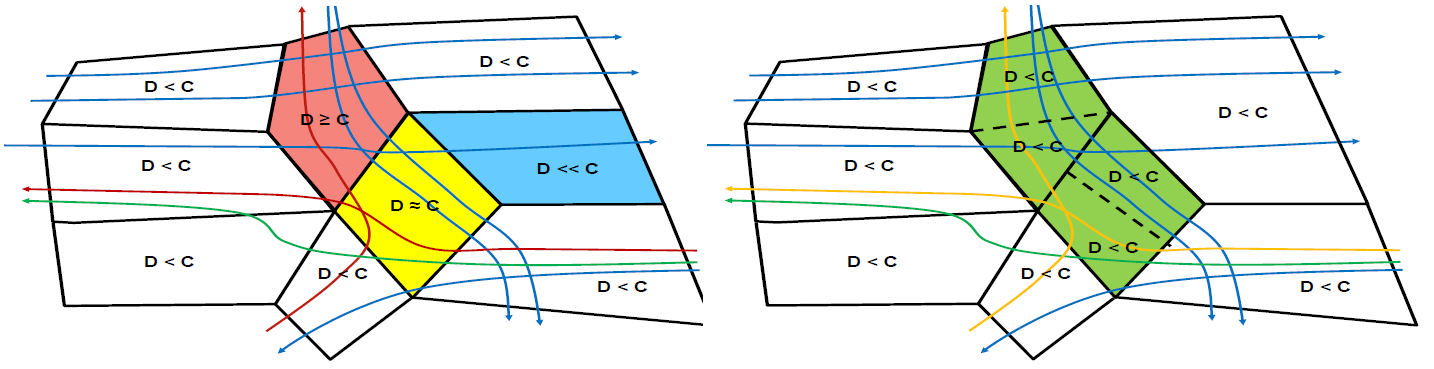
\includegraphics[width=1\textwidth]{\FIGDIR/02_02_DAM_Example}
    \caption{Example of DAM flight rerouting to homogenize traffic density \cite{gerdes2016dynamic}.}
    \label{fig:DAMExample}
\end{figure}

\begin{note}
    The airways cannot be changed, because the real-time change of airways is difficult. The change of cluster authority is possible because there are no changes for aircraft.
\end{note}

\noindent The airspace clusters are divided into three categories (fig. \ref{fig:DAMExample}):
\begin{enumerate}
    \item \emph{Under-fill} (blue) - there is fewer airplanes than its authority capacity.
    
    \item \emph{Saturated} (yellow) - there is enough airplanes to fill authority capacity.
    
    \item \emph{Over-fill} (red) - there are more airplanes than its authority capacity.
\end{enumerate}


\noindent The algorithm \cite{gerdes2016dynamic} will swap some airspace portions between neighboring authorities to balance the load (all authorities should be saturated in ideal conditions) (green) (fig. \ref{fig:DAMExample}).